\documentclass[oneside]{article}


\usepackage{textcomp}
%change font. (ALTERNATIVE:  mathpazo, mathptmx, helvet, avant, courier, chancery, bookman, newcent, charter)
\usepackage{charter} % math & rm 
\normalfont
\renewcommand{\ttdefault}{lmtt} %tt

\usepackage[utf8]{inputenc}
\usepackage[italian]{babel}
\usepackage[T1]{fontenc} % Use 8-bit encoding that has 256 glyphs
%\usepackage[latin3]{inputenc}
%\linespread{1.05} % Line spacing - Palatino needs more space between lines
\usepackage{microtype} % Slightly tweak font spacing for aesthetics
\usepackage[hmarginratio=1:1,top=32mm,columnsep=20pt]{geometry} % Document margins
\usepackage{multicol} % Used for the two-column layout of the document
\usepackage[hang, small,labelfont=bf,up,textfont=it,up]{caption} % Custom captions under/above floats in tables or figures
\usepackage{booktabs} % Horizontal rules in tables
\usepackage{float} % Required for tables and figures in the multi-column environment - they need to be placed in specific locations with the [H] (e.g. \begin{table}[H])
\usepackage{hyperref} % For hyperlinks in the PDF
\usepackage{lettrine} % The lettrine is the first enlarged letter at the beginning of the text
\usepackage{paralist} % Used for the compactitem environment which makes bullet points with less space between them
\usepackage{lipsum} % Package to generate dummy text throughout this template
\usepackage{graphicx}
\usepackage{enumitem}   

%abstract
\usepackage{abstract} % Allows abstract customization
\renewcommand{\abstractnamefont}{\normalfont\bfseries} 
\renewcommand{\abstracttextfont}{\normalfont\small} 

%titolo
\usepackage{titlesec} 
\renewcommand\thesection{\Roman{section}}
\renewcommand\thesubsection{\Roman{subsection}} 
\titleformat{\section}[block]{\Large\bfseries\scshape\centering}{\thesection.}{1em}{} 
\titleformat{\subsection}[block]{\large\scshape}{\thesubsection.}{1em}{} 
\titleformat{\subsubsection}[block]{\scshape}{\thesubsubsection.}{1em}{} 




%headers & footers 
\usepackage{fancyhdr} % Headers and footers
\pagestyle{fancy} % All pages have headers and footers
\fancyhead[L]{\bfseries{{\textsf{Davide Tedesco}}}}
\fancyhead[R]{\bfseries{{\textsf{$\bullet$ Verso una nuova frontiera della
 chitarra classica $\bullet$ }}}}
%\fancyhead[R]{\small \leftmark}
\cfoot{\thepage}




%----------------------------------------------------------------------------------------
%	TITLE SECTION
%----------------------------------------------------------------------------------------
\thispagestyle{empty}


\title{\vspace{-15mm}\fontsize{24pt}{10pt}\selectfont\textsf{\bfseries{\textsc{Verso una nuova frontiera della
 chitarra classica}}}} % Article title

\author{
\large
\textsc{Davide Tedesco}\\
\small{SMERM - Conservatorio di Musica di Roma, Santa Cecilia}\\
\small \href{mailto:me@davidetedesco.it}{\texttt{me[at]davidetedesco[dot]it}} 
%\vspace{-5mm}
}


\date{Luglio 2020}

%----------------------------------------------------------------------------------------




\begin{document}

\maketitle % Insert title

\tableofcontents

\thispagestyle{empty} 

%----------------------------------------------------------------------------------------
%	ABSTRACT
%----------------------------------------------------------------------------------------

\begin{abstract}

%\noindent
La composizione per strumento solo è andata negli anni via via accrescendosi, sia per le possibilità donate dall'arte musicale elettronica, che per l'interesse degli esecutori allo sviluppo di un nuovo linguaggio oltre quello che corrisponde al repertorio. Questo atteggiamento è particolarmente visibile nell'ambiente compositivo chitarristico, nel quale non solo compositori di professione, ma gli strumentisti stessi si sono iniziati a porre la questione del come potesse esser interpretata la loro performance all'interno di un discorso contemporaneo. La chitarra, che di per se si presta a vari utilizzi, viene dunque paragonata spesso a soli gesti virtuosistici che non nutrono un vero senso compositivo alimentando un discorso compositivo che porta la qualità dei manufatti musicali sempre più verso la semplicità e immediatezza di esecuzione. Il compositore contemporaneo deve quindi osservare l'ambiente che lo circonda notando e annotandosi i punti forza attuali ed estendendo le possibilità (che un esecutore) gli propone, Il seguente testo mira dunque all'apertura ad una ricerca scientifico-compositiva che cerchi di donare nuovo splendore alla chitarra classica, facendo render conto all'esecutore l'ampio spettro di possibilità sonore di cui è in potere ed ampliandolo attraverso l'utilizzo di adeguati mezzi elettronici.

\vspace*{4mm}
\end{abstract}


\hspace*{4mm}

%----------------------------------------------------------------------------------------
%	ARTICLE CONTENTS
%----------------------------------------------------------------------------------------
\newpage
\begin{multicols*}{2} % Two-column layout throughout the main article text



%-----------------------------------------------------1= Introduzione
\section{ Introduzione}

La chitarra è forse lo strumento che nelle varie epoche più si è adattato e piegato al volere e alla necessità di chi lo adoprava, esso è stato allo stesso tempo un mezzo popolare e colto che ha subito cambiamenti costruttivi sostanziali, ma mantenendo sempre la massima manegevolezza. Se nell’ambito colto venne molto apprezzato nel 1600,l’800 e dalla metà del 1900, in ambito popolare è divenuto forse lo strumento per eccellenza nel Novecento ed è stato oggetto di un boom di vendite (ancora in atto) e di apprezzamento, grazie alla sua mutevole e sempre interessante predisposizione all’incoronazione di miti pop grazie al sua versione elettrica, acustica etc... Lo strumento originario oltre le sue possibilità di esecuzione per mezzo di eccitazione delle corde è stato negli anni studiato e re-interpretato e ne sono conseguiti sviluppi multipli. Da un lato l’ambito percussivo è stato esplorato con brani quali \textit{Ko-Tha} di Scelsi e dall’altro l’amplificazione dello strumento acustico ha reso possibile l’emersione di timbriche e sonorità non percepibili(ascolto del microcosmo timbrico), facendo sviluppare notevolmente il fenomeno del \textit{tapping}\footnote{Visionato dal pubblico italiano per la prima volta in uno storico video che ritrae Vittorio Camardese, medico di professione, ma esperto di tapping per hobby} e della ricerca sulla sola tastiera. Numerosi sono inoltre gli utilizzi e le possibilità donate dall’elettrificazione e dal radicale re-styling, che portati all’interno della musica colta come mezzi post-avanguardistici hanno dato luogo quasi ad una corrente della chitarra elettrica contemporanea con autori quali Romitelli\footnote{Trash TV Trance, 2002}  e Murail\footnote{Vampyr!, 1984}  ad esempio. 
La domande che sorgono da una prima panoramica sono: qual’è il ruolo della chitarra (classica, elettrica ed in tutte le sue versioni) nella musica contemporanea oggi? Essa è ancora uno strumento attuale? Quale deve essere l’atteggiamento del compositore verso uno strumento usato tanto per il suo repertorio popolare, quanto per il suo repertorio classico? Questo breve testo cerca di esplicare e trarre spunto ed approfondire alcuni aspetti portando la chitarra classica nel presente ed ripensando l’elettrificazione della stessa e la necessità di un’operazione del genere. 


%----------------------------------------------------2= La chitarra

\section{ Breve storia della chitarra}

Dalla famiglia dei liuti nel 500 d.C. circa, si iniziarono ad intravedere alcune delle più moderne versioni dello strumento con il guscio (la cassa armonica) non più di forma tondeggiante, ma esso fu sostituito da due superfici piatte unite da una fascia.

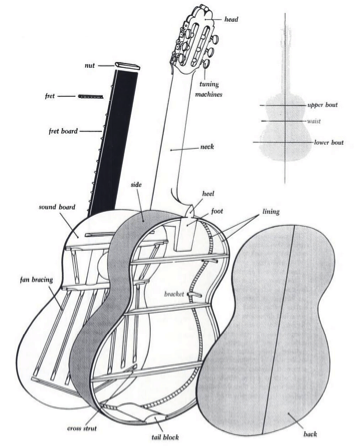
\includegraphics[width=0.4\textwidth]{img/chit_spaccato.png}

Anche se l’origine della chitarra ci indica che essa provenga dal liuto, il tempo l’ha portata con sé fino ai giorni nostri, e questo strumento attraversando i secoli ha cambiato varie volte nome e già nel XIV secolo troviamo il nome di chitarra moresca in un libro spagnolo, che variando nome, venne chiamata in seguito mandola.
Questi strumenti a corda pizzicata attraverso un plettro od una penna ebbero spesso quattro corde a simboleggiare le quattro fasi della luna, le settimane del mese e via discorrendo, gli accordi, o in ogni caso il modo di suonare simultaneamente più corde era in quel periodo sconosciuto ai più, e lo strumento era suonato inizialmente solamente per eseguire una melodia ed occasionalmente vi venivano eseguiti degli ostinati per accompagnare questa melodia, con il passare dei secoli e dei luoghi in cui lo strumento fu portato e sviluppato, le sapienze orientali e occidentali si mescolarono fino a renderlo in Andalusia il liuto che conosciamo.
Il liuto divenne lo strumento predominante in Europa tra 1500 e 1700, anche se in quel periodo in Spagna non era molto apprezzato ed utilizzato dall’aristocrazia, la musica popolare spagnola fece invece conoscere la chitarra al resto d’Europa. Benché la musica colta veniva invece eseguita su di una vihuela, in genere la vihuela da mano, che si differenziava dalla vihuela da arco per il modo in cui la si suonava, la vihuela da mano aveva 6 o 7 corde ed era accordata in vari modi.
L’arte liutistica ebbe il suo declino verso la fine del ‘600 quando strumenti come il clavicembalo molti altri strumenti a tastiera iniziarono a prendere piede, ma con il declino del liuto la  chitarra inizió ad essere più apprezzata, soprattutto per la sua maneggevolezza e facilità di trasporto.
Sui principi del 600 la chitarra aveva solamente quattro corde doppie, che erano accordate spesso  “Do-Fa-La-Re” o “Fa-Si-Re-Sol”. 
In questo periodo la chitarra aveva la cassa armonica più stretta e profonda.
La chitarra italo-spagnola incominciò a viaggiare in Europa arrivando prima di tutto all’aristocrazia francese, e venne raffigurata più e più volte in affreschi alla corte francese.
La chitarra divenne dunque uno strumento da dilettanti e fu semplificata, sei corde singole e non più doppie con accordatura “Mi-La-Re-Sol-Si-Mi”, ovvero l’accordatura tradizionale che abbiamo ancora oggi.
Il nuovo modello di chitarra era dunque maturo e divenne più facile da maneggiare. Nell’800 venne poi introdotta un’altra miglioria con la sostituzione dei piroli in legno con quelli a viti in metallo.
La chitarra ebbe alti e bassi nella sua diffusione e per il suo gradimento generale e furono divisi fino al  primo ‘900 per ambito colto e popolare.
Essa fu riportata, in ambito colto, a dei livelli altissimi grazie all’apporto di figure come Andrés Segovia, Joaquin Rodrigo e Heitor Villa-Lobos.


%----------------------------------------------------3= La chitarra nella musica contemporanea

\section{ La chitarra nella musica contemporanea}

Iniziando a scavare all'interno della storia della composizione per questo strumento, non si puó far altro che passare per i classici oramai intramontabili che ogni studente di Conservatorio incontra ed oltre ai già nominati Segovia, Rodrigo e Villa-Lobos, ci si ritrova ad osservare scaffali interi dei negozi in cui si sono inseriti centinaia di studi per chitarra di autori quali: Sor, Giuliani, Carulli e via dicendo. Non dobbiamo dunque stupirci al fatto che in sede di concerto il chitarrista tenda a realizzare una gara \textit{all'esecuzione piú veloce}, poichè la premessa didattica è sempre stata improntata alla ricerca della velocità di esecuzione ed alla perfezionamento del virtuosismo. Laddove invece si trovano degli esecutori in grado di interpretare e contestualizzare un'opera si trovano invece delle gemme, che riescono veramente a far prender forma alle composizioni per chitarra sola. Ne sono esempi Elena Casoli\footnote{Milano, 1962}, Arturo Tallini\footnote{Napoli, 1958} e Ruben Mattia Santorsa\footnote{Potenza,1992}, oltre a molti altri nel panorama internazionale, che attraverso la collaborazione proficua con compositori, alunni e conservatori riescono a delineare dei progetti dal piú vasto respiro ed a donare uno spazio per la chitarra all'interno della \textit{giungla} musicale odierna.
%\begin{figure}
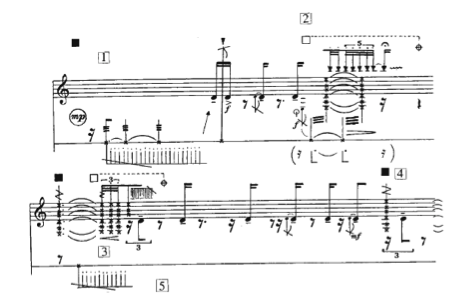
\includegraphics[width=0.5\textwidth]{img/ektopos.png}
%\caption{Agostino Di Scipio - Ektopos}
%\label{img/ektopos.png}}
%\end{figure}
L'ambiente chitarristico rivela dunque alcune dei suoi gioielli proprio attraverso degli esecutori che sono riusciti a comprendere il ruolo che il proprio strumento può avere e ponendosi con occhio ed orecchio vigile allo studio delle partiture contemporanee. Se da un lato ci si aspetterebbe un vasto repertorio chitarristico contemporaneo ricco di idee e nuove possibilità, da un certo punto di vista si rimane delusi, trovando opere realizzate da grandi e rinomati compositori quali Berio\footnote{Sequenza XI}, Ferneyhough\footnote{No time} e Maderna\footnote{Y Después}, che rispecchiano però un'idea di composizione \textit{novecentesca}. Si trovano invece spunti di riflessione brillanti in compositori a noi piú vicini come Di Scipio\footnote{Ektopos, in figura}, Murail\footnote{Tellur} e Romitelli\footnote{Solare, Seascape ed altre opere}. Sebbene queste composizioni riescano in ogni modo a dar giustizia alle sei corde, troviamo nel brano di Scelsi \textit{Ko-Tha}\footnote{del 1962} una piú vasta ricerca sul suono ed una prima esperienza chitarristica percussiva che cerca di sfruttare lo strumento in maniera non convenzionale. Dall'ascolto delle registrazioni \textit{scelsiane} custodite alla \textit{Fondazione Isabella Scelsi} notiamo dunque una vera e propria ricerca del e sul suono che si avvicina al microcosmo timbrico piú di quanto altri compositori dopo di lui sono riusciti a fare. Dunque l'utilizzo dello strumento come una percussione, degli strappati e delle possibilità al di fuori del melodico iniziano veramente a ristrutturare la concezione compositiva dello strumento. La ricerca e la risposta di Berio è invece (come in tutte le sue sequenze) una \textit{creazione di un virtuosismo} che punta al far esperire lo strumento e le sue capacità melodico-armoniche al massimo delle sue possibilità. 
Se dunque l'utilizzo della chitarra classica all'interno dell'ambito contemporaneo riesce in qualche modo a tagliare la tela della tradizione, le esperienze menzionate in precedenza di interventi musicali con la chitarra elettrica, entrano possentemente all'interno del paesaggio musicale, rendendo ben visibili le possibilità timbriche, compositive e teatrali che uno strumento popolare quanto diffuso puó realizzare. Non è un caso che le composizioni per chitarra elettrica di Murail e Romitelli siano costantemente suonate, proposte e pubblicate sul web. 
Se dunque questo lo strumento \textit{rivisitato} è riuscito a portare tanta novità e apprezzamento, perchè la chitarra classica rimane sempre piú nell'ombra del panorama colto?
L'utilizzo dell'elettronica all'interno del panorama musicale tradizionale per strumento solo è come se sia vista come un di piú, da poter incollare accanto o come sfondo al suono dello strumento solo, rendendo di fatto pochissime composizioni per chitarra classica ed elettronica sensate.

%----------------------------------------------------4= L’aumentazione: l'amplificazione, Il feedback e la distorsione

\section{ L’aumentazione}

In questo vasto ambiante compositivo ed esecutivo che porta con se brillantezza e freschezza di idee, vi è però sempre un minimo comun denominatore, ovvero lo strumento solo lasciato alle sue possibilità fisiche che oramai ha reso stereotipato il modo di scrivere per esso. Forse si puó notare nella mancanza dell'elettronica all'interno del discorso compositivo chitarristico classico, una voglia di legame con il passato che sta portando a lungo andare alla dispersione dei risultati raggiunti nel '900, lasciando lo strumento in mano alla sola musica popolare. 

\noindent Da queste riflessioni nasce dunque la necessità di provare a realizzare un qualcosa che possa integrare l'elettronica con lo strumento, come è già stato fatto per molti altri strumenti soli, riuscendo a captare il microscopico dello strumento, le caratterizzazioni fisiche dello strumento e le possibilità donate dall'esperienza della chitarra elettrica nel contemporaneo. Il processo che nasce da questi pensieri può esser inteso come una vera e propria \textit{aumentazione} dello strumento stesso che attraverso l'elettronica e la gestione del gesto musicale per mezzo dell'elettronica riesce a donare nuove possibilità allo stesso. La ricerca in atto porta dunque alle prime tre possibilità che il sistema realizzato mette a disposizione: 
\begin{enumerate}[label=(\roman*)]
\item L'amplificazione
\item Il feeback 
\item La distorsione
\end{enumerate}

\subsection{L'amplificazione} 
Il posizionamento di un microfono piezo-elettrico sul \textit{piano armonico} dello strumento è un'operazione non nuova nell'ambito chitarristico. Laddove esso viene utilizzato come mero sistema per fare uno zoom sullo strumento in situazioni in cui lo stesso risulterebbe flebile ed impercettibile, esso viene utilizzato solamente come mezzo di amplificazione puro che ad un livello di amplificazione costante porta il suono chiaramente agli spettatori. La soluzione tecnica non porta con se però l'esperienza che Stockhausen\footnote{in Mikrofonie I} ha elaborato, lasciando le possibilità che un'azione del genere procura nel dimenticatoio. Infatti, l'utilizzo di un sensore a contatto e la gestione dello stesso in tempo reale è forse il modo piú immediato, chiaro e apprezzabile di operazione dell'osservazione del microscopico.

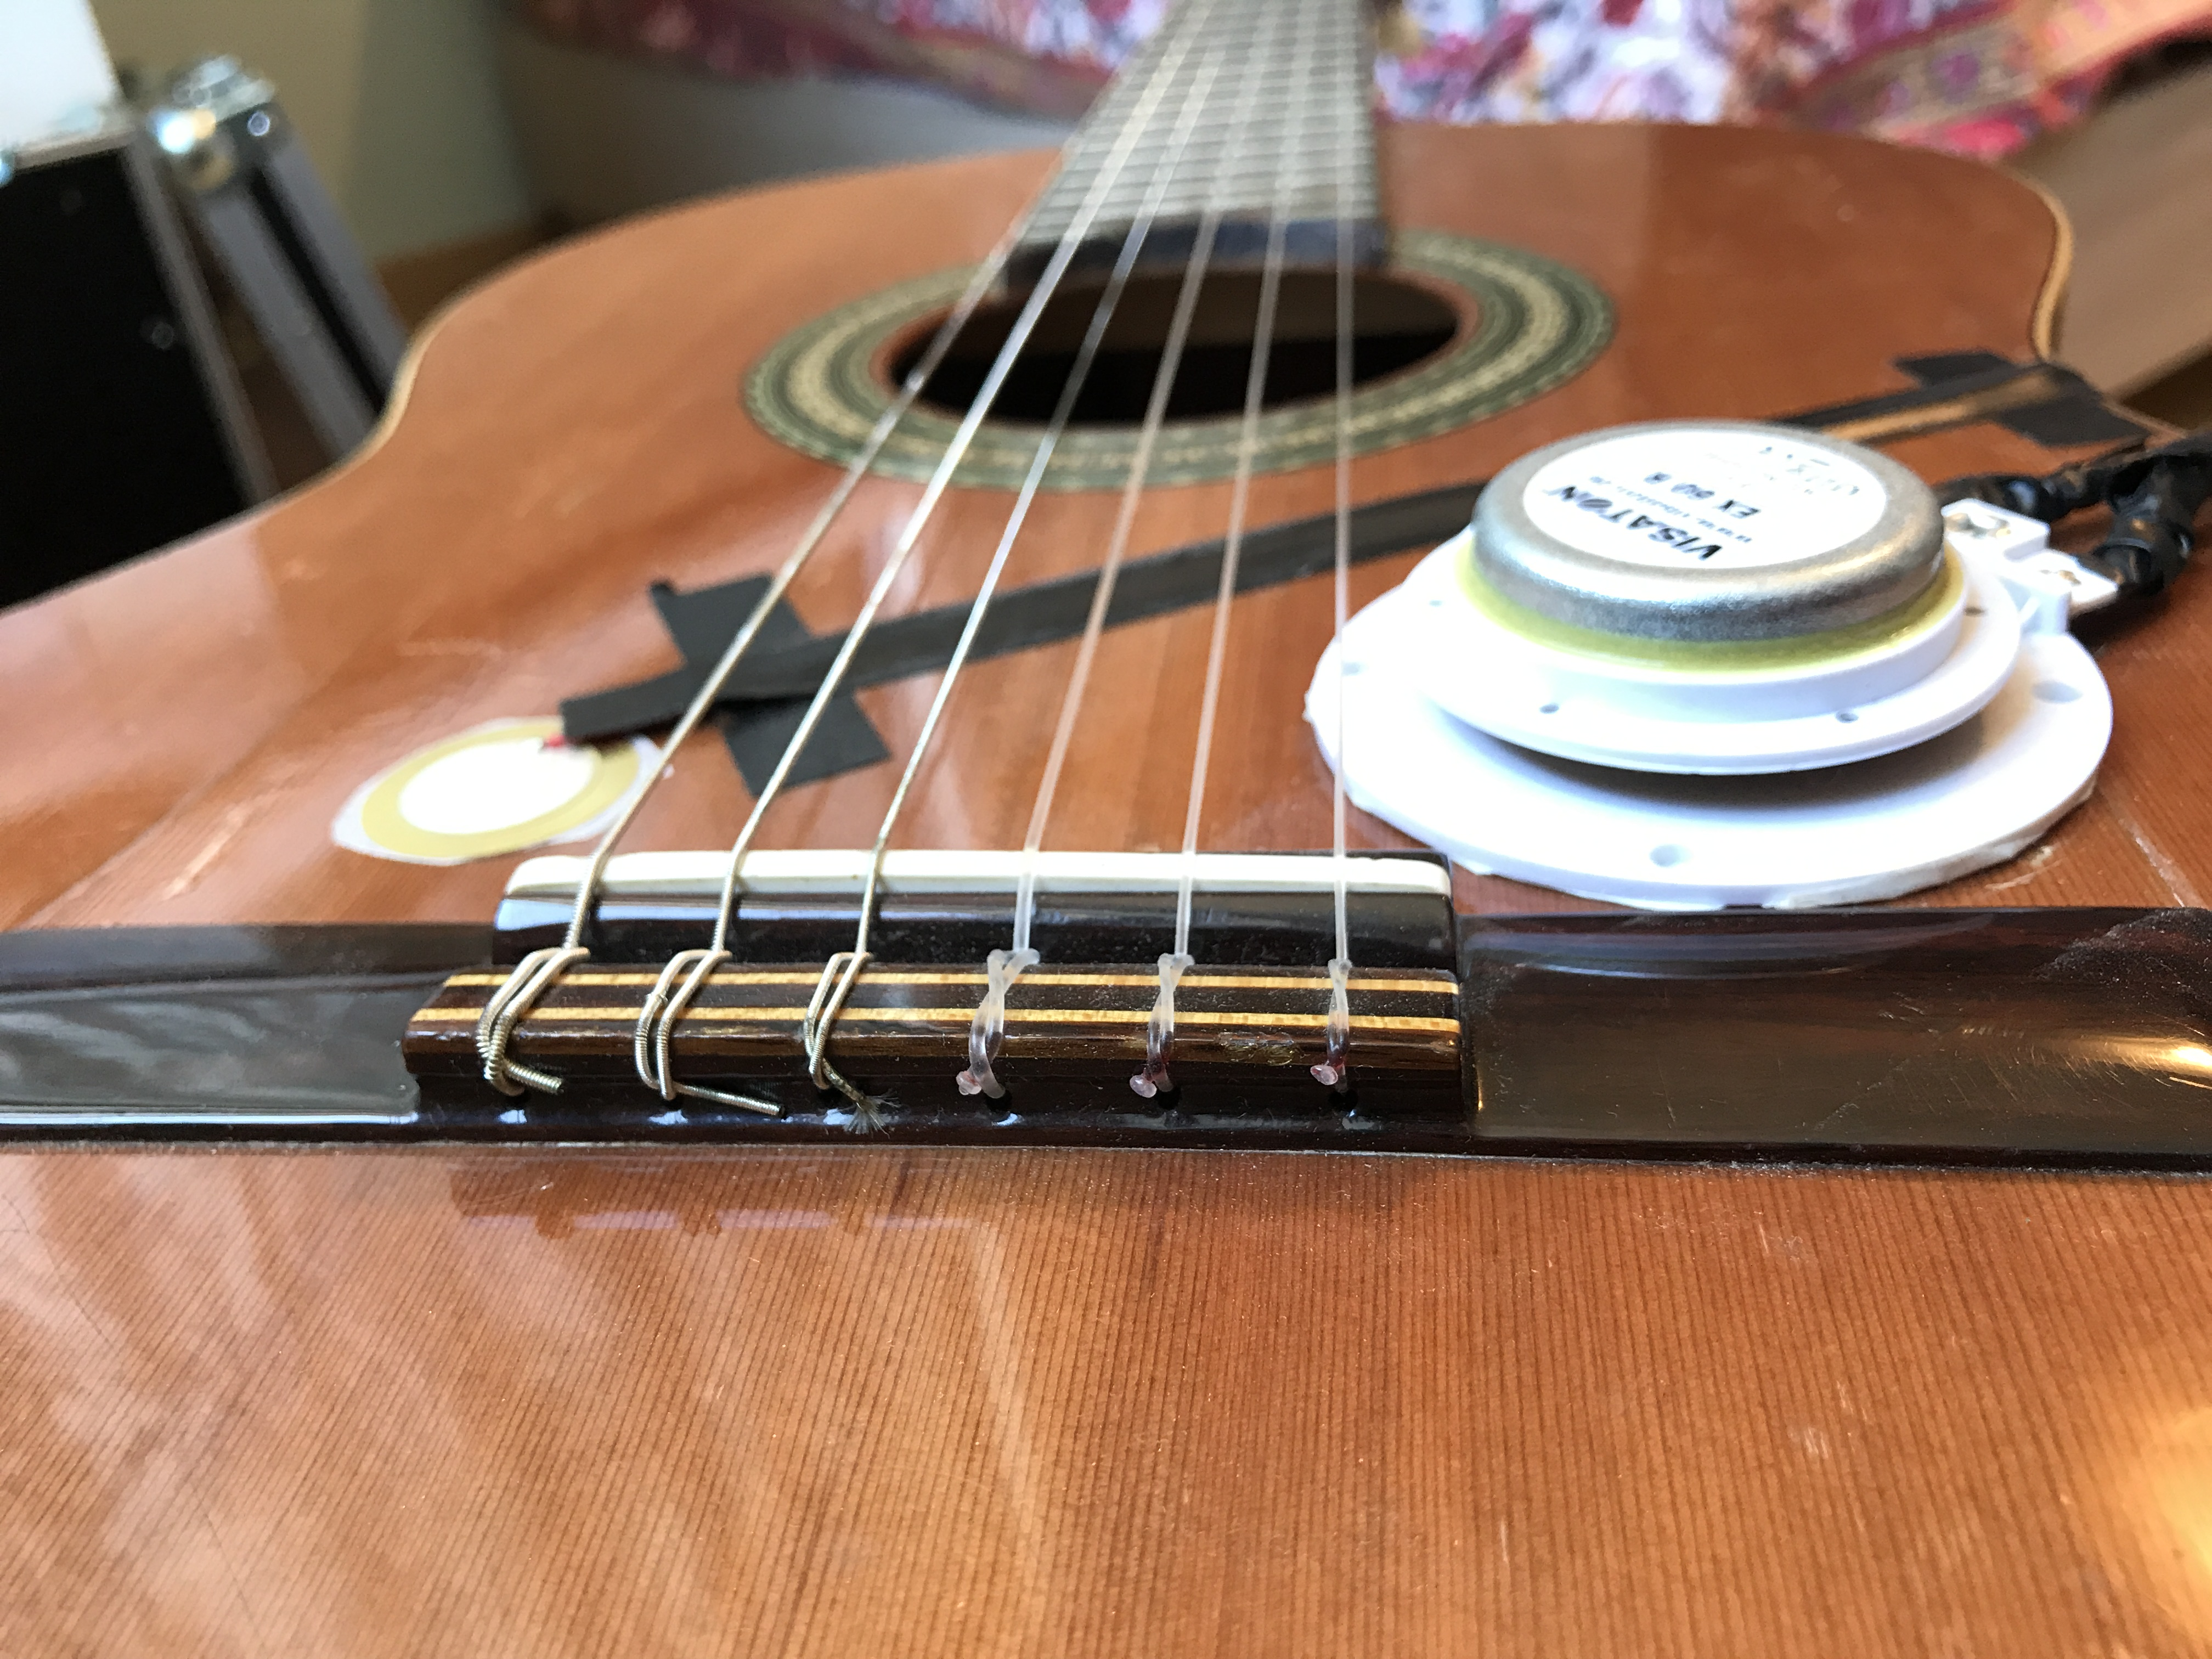
\includegraphics[width=0.4\textwidth]{img/chit.jpg}

Le unghie, i polpastrelli ed il palmo della mano sono eccitatori talmente vari che è possibile apprezzarne chiaramente la differenza solamente attraverso l'amplificazione, rendendo chiaro ciò che già da un paio di metri di distanza in ambito chitarristico è considerato impossibile. La gestione inoltre attraverso il filtraggio del suono in tempo reale rende ancor meglio l'idea di cosa due strumenti(la chitarra ed il microfono) possano realizzare, donando veramente nuove sonorità e timbriche allo strumento chitarra, senza appiattirsi alla importante ma pur limitata esperienza polpastrello-unghia descritta da Pujol\footnote{Emilio Pujol, El dilemmma del sonido en la guitarra, Ricordi 1979}.

\subsection{Il feedback} 
Da anni utilizzata come tecnica di aumentazione nell'ambito elettrico della chitarra, ma seppur classificabile in diverse tipologie è forse una delle frontiere da esplorare nell'ambiente musicale chitarristico classico. Il feedback classificabile in diverse tipologie\footnote{feedback digitale, feedback di natura acustica, feedback di natura strutturale}, può essere implementato strutturalmente sullo strumento per mezzo di 2 componenti: un sensore ed un attuatore\footnote{altoparlante senza membrana in grado di propagare strutturalmente il suono}. Essi realizzano un vero e proprio sistema di feedback strutturale gestibile dall'esecutore che è limitato solamente dalla natura fisica dello strumento che viene utilizzato. Attravero una IR\footnote{risposta all’impulso, ovvero fotografia di come reagisce un corpo risonante ad un impulso} riusciamo dunque a determinare le zone frequenziali in cui il sistema potrebbe rispondere meglio alle sollecitazioni effettuate da particolari frequenze.
\newline

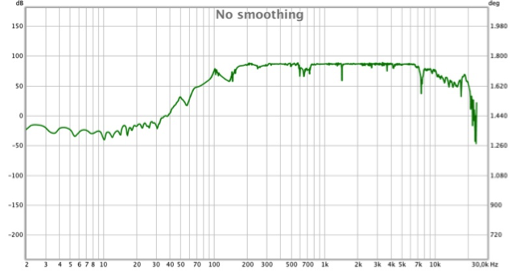
\includegraphics[width=0.4\textwidth]{img/ir.png}

Nell'immagine esemplificativa notiamo la curva della risposta in frequenza del sistema in quella che chiameremo \textit{posizione 1}, ovvero l'accoppiamento di sensore e attuatore in due precisi luoghi. Come è possibile visionare nel video esemplificativo\footnote{\href{https://www.youtube.com/watch?v=7BwwTopM3Ek}{Link al video d'esempio della gestione del feedback}}, la gestione del feedback sullo strumento risulta adeguata a seconda dei movimenti dell'esecutore, i quali catalogati e studiati rientreranno all'interno dei gesti da implementare in partitura, facendo raggiungere una nuova consapevolezza dello strumento al musicista. I primi limiti che si pongono con il feedback sono però le frequenze a cui lo strumento riesce a risuonare(dipendenti dallo strumento e dal sensore ed attuatore utilizzati), i quali vengono però aggirati semplicemente dall'implementazione di filtri che rendono piú malleabile l'utilizzo del feedback stesso. La tipologia di filtro va ovviamente a denotare caratteristiche diverse nella realizzazione sonora-timbrica, ma non potrà mai realizzare un qualcosa di totalmente estraneo alla fisicità dello strumento in uso, ciò renderà sicuramente ogni esecuzione unica, ma denotando un unico luogo di provenienza compositiva.

\subsection{La distorsione} 
Dopo aver realizzato che la chitarra può dunque essere aumentata riuscendo a far espletare nuove sonorità, timbri e metodologie di esecuzione si è pronti al passo successivo, ovvero cercare di far appropriare lo strumento originario delle tecniche e delle possibilità della chitarra elettrica. Nell'esempio video al piè\footnote{\href{https://www.youtube.com/watch?v=K3yqyxcJStg}{Link al video d'esempio della distorsione}} si nota come l'implementazione e la gestione della distorsione sia non solo possibile e funzioni molto bene, ma come essa riesca a portare un elemento come quello della distorsione, naturalmente nel contesto chitarristico. La chitarra di per sè è infatti ora equipaggiata delle possibilità che la chitarra elettrica detiene(attraverso il sensore piezo-elettrico), e la distorsione come mezzo espressivo riesce a fondere la tecnica e i timbri sviluppati nell'ambito popolare degli ultimi 100 anni con le consuetudini e le corde in nylon della chitarra classica. Questo ultimo passaggio all'interno del discorso di \textit{aumentazione} dello strumento svecchia notevolmente le possibilità ed insieme al feedback ed alla \textit{microfonazione compositiva} dona nuova linfa ad uno strumento storico e storicizzato.


%\vfill\null
%\columnbreak
%----------------------------------------------------5= Gli Sketches e gli Studi per chitarra
\section{ Gli Sketches e gli studi per chitarra}
Alla ricerca non di un nuovo strumento, ma bensí di una nuova tipologia di scrittura e ricerca di un nuovo virtuosismo, non basato sulla sola velocità dell’esecuzione dei brani, e  sfruttando l'\textit{aumentazione} appena descritta si giunge allo sviluppo dei primi esempi compositivi.
Il primo approccio in questo percorso è consistito nella realizzazione di \textit{Sketches}\footnote{\href{https://github.com/SMERM/BN-Tedesco/blob/master/COME-02/Lezioni_in_Compresenza/20200324/Sketches.pdf}{Link agli Sketches}}, ovvero degli appunti con delle prime idee che potevano essere implementate sullo strumento prima dell'implementazione del sistema elettroacustico. Con esse è sorte alcune questioni puramente di scrittura sul \textit{come} rappresentare chiaramente i movimenti delle due mani, i \textit{luoghi percussivi} sulla chitarra ed il rapporto con l'elettronica.
La scrittura per mezzo di due pentagrammi ha reso perfettamente il senso di contemporaneità dei gesti fra le mani, fungendo per la mano sinistra da pentagramma tradizionale, mentre per la mano destra da una intavolatura\footnote{essa veniva utilizzata nel passato come metodologia di scrittura liutistica, ed oggi è usata per imparare a suonare}. 

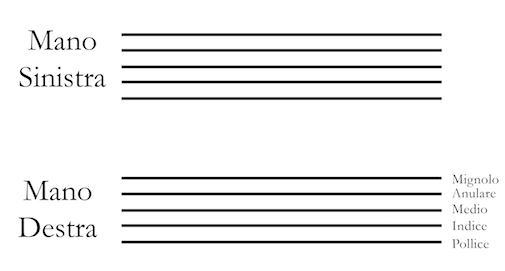
\includegraphics[width=0.4\textwidth]{img/legenda.png}

L'intavolatura per la mano destra riporta dei luoghi numerati sul piano armonico(in figura) che possono esser combinati con le dita o parti della mano destra. In questa intavolatora i cinque righi vengono utilizzati per le cinque dita della mano. 

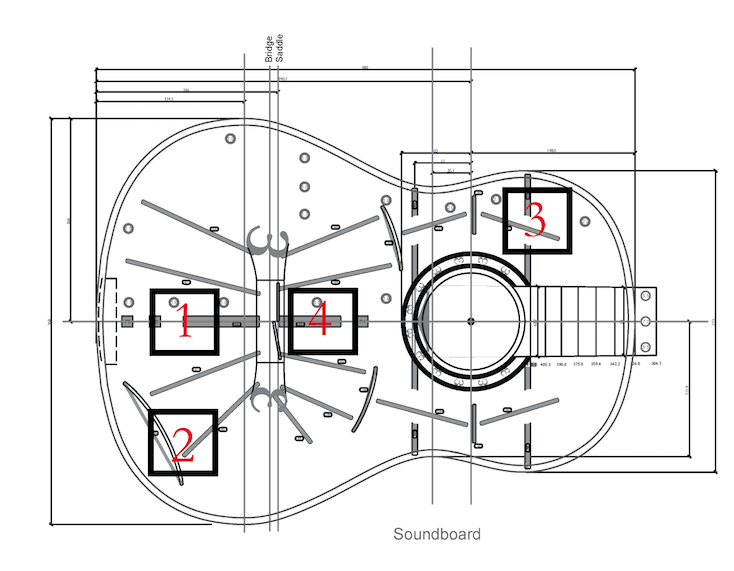
\includegraphics[width=0.4\textwidth]{img/luoghi_perc.png}

I \textit{luoghi percussivi} numerati sono molto diversi dal punto di vista della resa percussiva ed hanno spettri frequenziali variegati utilizzabili a seconda della necessità possono essere cosí descritti :
\begin{enumerate}
\item $\longrightarrow$Profondo e risonante 
\item $\longrightarrow$Rotondo e risonante
\item $\longrightarrow$Secco e medio-alto
\item $\longrightarrow$Chiaro e deciso(il piú utilizzato poichè capace di far risuonare le corde percuotendole al ponte)
\end{enumerate}

L'esperienza degli \textit{Sketches} ha fatto nascere delle prime risposte compositive all'interno degli \textit{Studi} per chitarra sola, che riportano a livello pratico alcune delle esperienze avute durante l'importante periodo di ricerca. Essi ad oggi sono quattro e riportano 4 tipologie di timbrica e realizzazione diversa.
L'importanza della scrittura di studi, che nella storia della musica sono interpretati a livello compositivo molto vario(dagli studi prettamente tecnici a quelli totalmente compositivi e intrisi di sperimentazione della scrittura), fa si che l'interprete divenga sempre piú consapevole, a piccoli passi, della totalità di prospettive sonore disponibili e velate nel suo strumento. All'interno di questo progetto di molto ampio respiro, il \textit{primo studio}\footnote{\href{https://github.com/SMERM/BN-Tedesco/blob/master/COME-02/Lezioni_in_Compresenza/20200331/Draft_1_Studio_n.1_Audio.wav}{Link all'audio}} non fa uso dell'elettronica ma bensí della voce dell'interprete, lasciando trasparire una volontà di ricerca all'interno dell'interprete insieme a quella all'interno dello strumento. Nel \textit{secondo studio}\footnote{\href{https://github.com/SMERM/BN-Tedesco/blob/master/COME-02/Lezioni_in_Compresenza/20200407/Draft_1\%20Studio\%20n.2\%20Partitura.pdf}{Link alla partitura}} l'amplificazione viene utilizzata per la prima volta in combinazione con il sensore e l'attuatore oltre che per l'amplificazione viene utilizzato come un emettitore di suono. È però nel \textit{terzo}\footnote{\href{https://github.com/SMERM/BN-Tedesco/blob/master/COME-02/Lezioni_in_Compresenza/20200519/Appunti_Studio_n.3_a.jpeg}{Link agli appunti del terzo studio}} e \textit{quarto studio}\footnote{\href{https://github.com/SMERM/BN-Tedesco/blob/master/COME-02/Lezioni_in_Compresenza/20200616/Studio_n.4_a.pdf}{Link alla partitura}} che il feedback inizia a presentarsi nella sua potenza espressiva. La distorsione del terzo studio ed il Feedback oltre che la scordatura denotano degli elementi in piú che l'interprete deve studiare e capire come realizzare al meglio proiettando nella nuova tipologia di scrittura.

Questi studi non ancora ultimati ed incentrati quasi alla sola \textit{ri-}scoperta dello strumento, divengono dunque il punto di partenza di un percorso complesso assieme all'interprete, facendolo porre con spirito critico ed un pizzico di fantasia di fronte a nuove prospettive. Queste possibilità e nuove proposte (forse non proprio alla portata di tutti) cercheranno dunque di render giustizia nuovamente allo strumento, che risponderà in modo opportuno laddove lo strumentista saprà carpirne il comportamento. %----------------------------------------------------6= Conclusioni

\section{ Conclusioni \& nuove prospettive}

Dal lavoro di ricerca effettuato sorgono, oltre a notevoli ed importanti traguardi per la composizione chitarristica anche delle perplessità. 
Nell’utilizzo di uno strumento come la chitarra la standardizzazione nella costruzione dello strumento è sempre stata un qualcosa che i costruttori non hanno voluto attuare, rendendo di fatto totalmente diverse le costruzioni e le caratteristiche fisiche interne dello stesso. Esse fanno si che l'implementazione di un qualsiasi apparato su di esse e l'utilizzo del corpo della chitarra con metodologie elettroniche debba essere attento ed accurato per ottenere i risultati richiesti. Come è possibile notare nella figura sottostante, sono infatti multiple le metodologie di \textit{catenatura}\footnote{da catene, steli in legno che collegano le varie zone del piano armonico} della chitarra che non rendono uniforme la moltitudine degli strumenti ad oggi costruiti.


\includegraphics[width=0.4\textwidth]{img/catene.png}

Da ciò ne deriva che un importante apporto è quello dello strumentista che in vece del compositore ed tenendo a mente il suo obiettivo finale (ovvero la buona riuscita del brano) deve studiare la metodologia piú appropriata per il posizionamento e la buona riuscita dello stesso. Si propone dunque di allegare al brano stesso delle caratteristiche fondamentali che il posizionamento di attuatore e sensore devo far risaltare, rendendo cosí giustizia alle composizioni che ne fanno uso. Attreverso strumenti come le figure di Chladni\footnote{tecnica che grazie alla vibrazione di una lastra permette di visualizzare i punti nodali della stessa, ovvero quei punti in cui l'ampiezza della vibrazione è virtualmente nulla} si puó ad esempio effettuare la ricerca dei punti nodali dello strumento, rendendo il lavoro più semplice allo strumentista, ma ogni strumento avrà dei suoi punti che faranno espletare al meglio risultati analoghi. Bisogna quindi precisare che la ricerca in questa direzione cercando di sfruttare lo strumento nel miglior modo possibile dovrà esser seguita dal compositore e che egli dovrà fornire degli strumenti adeguati per far preparare lo strumentista all'esecuzione in concerto. Questi strumenti saranno un vero è proprio mezzo pratico che dovranno accompagnare nella messa in scena e preparando lo strumento e l'interprete all'esecuzione.


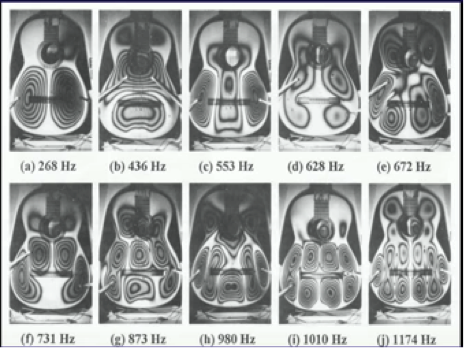
\includegraphics[width=0.4\textwidth]{img/chladni1.png}

Si punta quindi ad una ricerca da parte dello strumentista che possa far trasparire l'intenzione compositiva anche attraverso strumenti realizzati costruttivamente in maniere differenti, anche se come al solito la ricerca di un metodo chiaro di scrittura è inoltre il punto fondamentale del discorso su di un nuovo metodo di scrittura del suono e della produzione dello stesso. Allo stato attuale la mancanza di trasparenza influisce negativamente su ogni aspetto musicale avvenuto dopo l'approfondita ricerca su di uno strumento, mentre ci si propone di sviluppare documentazione tale da chiarire ogni dubbio dell'esecutore ogni qualvolta esso si presterà all'eseguire la composizione. È dunque il rapporto di fiducia tra il compositore e l'interprete che lega la buona riuscita a un qualcosa di totalmente nuovo ma con forti radici nella tradizione e solo attraverso una responsabilizzazione dell'esecutore nella prima fase di conoscenza del nuovo modo di scrivere egli si potrà istruire all'essere più sensibile ed ascoltare il proprio strumento. All'interno di questa prospettiva intrisa di serietà e scrupolosità nel perseguire un obiettivo la gestione dell'amplificazione o del feedback da parte dell'esecutore per mezzo di un pedale resistivo può far veramente responsabilizzare lo stesso, facendogli render conto della potenza e del controllo che non solo con le mani ma anche con i piedi puó avere sul suono, permettendo al compositore di delegare il Live Electronics quasi interamente al musicista, e lasciando di fatto invariata la figura iconica del chitarrista solo sul palco, che puó di fatto gestire autonomamente ed interamente la parametrica complessiva del brano.

Le nuove prospettive pongono dunque nuovi limiti e nuove possibilità, ed ora potendo sfruttare l'attuatore posizionato sullo strumento è facile realizzare il passaggio concettuale che pone la riproduzione del suono attraverso lo stesso. È piú complesso comprendere e capire cosa poter diffondere sul piano armonico dello strumento e conseguentemente nel sistema realizzato, cercando di sfruttare al massimo il sistema ora disponibile; nel corso di questa prima parte di ricerca si è implementato  ad esempio  l'algoritmo del Karplus-Strong\footnote{Kevin Karplus, Alex Strong, \emph{Digital Synthesis of Plucked-String and Drum Timbres},Computer Music Journal, Vol. 7, No. 2, Summer 1983} che diffuso dall'attuatore ha reso ancor piú veritiera la resa acustica finale dello stesso\footnote{\href{https://github.com/SMERM/BN-Tedesco/tree/master/COME-02/Lezioni_in_Compresenza/20200331/Esempi_Karplus-Strong_Attuatore_su_chitarra}{Alcuni esempi del Karplus-Strong applicato al piano armonico}}.

Il compositore è dunque chiamato a selezionare e smistare le sue idee confrontandole il piú scientificamente con le possibilità che lo strumento gli dona, ciò è però reso possibile solamente da un attenta ed oculata scelta dei passi da compiere lungo il percorso di ricerca, che oltre a completare e rendere consapevole di ciò che egli può realizzare. Se dunque è vero che il percorso verso una nuovo modo di comporre è lungo e pieno di impervie, quale può mai essere il miglior modo di affrontarle se non insieme ad un interprete? Si vuole quindi sottolineare attraverso ciò l'importanza nella ricerca necessaria sullo strumento e ricordando le parole di Segovia: \begin{quote} La chitarra è lo strumento più semplice da suonare ma il più difficile da suonare molto bene. \end{quote} Si intende quindi molto chiaramente come questo strumento abbia potuto spopolare in una miriade di contesti, portandosi dietro sempre il fascino di una donna e la possenza masculina delle sue corde piú gravi, passando per corti, auditorium e concerti da migliaia di persone e pur celando  dentro di sé sempre nuove possibilità. 


\newpage

%===============================================Brani ascoltati e partiture visionate

\section{ Brani ascoltati \& partiture visionate}
•\textsc{\textsf {Agostino Di Scipio}}, \emph{Ektopos}, UT Orpheus 2000\\
•\textsc{\textsf {Azio Corghi}}, \emph{Consonancias y Redobles}, Universal Edition 1973\\
•\textsc{\textsf {Barbara Kolb}}, \emph{ - Looking for Claudio}, Boosey \& Hawkes 1975\\
•\textsc{\textsf {Benjamin Britten}}, \emph{Nocturnal After John Dowland}, xx 199x\\
•\textsc{\textsf {Brian Ferneyhough}}, \emph{Kurze Schatten II}, xx 199x\\
•\textsc{\textsf {Brian Ferneyhough}}, \emph{No time}, xx 199x\\
•\textsc{\textsf {Bruno Maderna}}, \emph{Y Después}, xx 199x\\
•\textsc{\textsf {Bruno Maderna}}, \emph{Serenata per un satellite}, Ricordi 1969\\
•\textsc{\textsf {Fabio Vacchi}}, \emph{Plynn}, xx 199x\\
•\textsc{\textsf {Fabrizio Casti}}, \emph{ L' 'Anima Visionaria}, UT Orpheus 2000\\
•\textsc{\textsf {Fausto Romitelli}}, \emph{Trash TV Trance}, Ricordi 2002\\
•\textsc{\textsf {Fausto Romitelli}}, \emph{Solare}, Ricordi 1984\\
•\textsc{\textsf {Fausto Romitelli}}, \emph{La lune et les eaux}, Ricordi 1991\\
•\textsc{\textsf {Fausto Romitelli}}, \emph{Seascape}, Ricordi 1994\\
•\textsc{\textsf {Fausto Romitelli}}, \emph{Coralli}, Ricordi 1987\\
•\textsc{\textsf {Fausto Romitelli}}, \emph{Highway to hell}, Ricordi 1984\\
•\textsc{\textsf {Federico Bonacossa}}, \emph{Shikantaza}, Cyklos 2005\\
•\textsc{\textsf {Franco Donatoni}}, \emph{Algo}, xx 199x\\
•\textsc{\textsf {Giacinto Scelsi}}, \emph{Ko-Tha}, Salabert 1962\\
•\textsc{\textsf {Helmut Lachenmann}}, \emph{Salut für Caudwell}, xx 199x\\
•\textsc{\textsf {Luciano Berio}}, \emph{Sequenza XI}, Universal Edition 1988\\
•\textsc{\textsf {Maurizio Pisati}}, \emph{Set7}, Kairos 2017\\
•\textsc{\textsf {Sylvano Bussotti}}, \emph{Ultima rara,}, xx 1969\
•\textsc{\textsf {Tristan Murail}}, \emph{Tellur}, xx 1977\\
•\textsc{\textsf {Tristan Murail}}, \emph{Vampyr!}, xx 199x\\
•\textsc{\textsf {Toru Takemitsu}}, \emph{12 songs for guitar}, Schott 2005\\
•\textsc{\textsf {Toru Takemitsu}}, \emph{All In Twilight}, Schott 1993\\
•\textsc{\textsf {Toru Takemitsu}}, \emph{Equinox}, Schott 1993\\
•\textsc{\textsf {Toru Takemitsu}}, \emph{To the edge of dream}, xx 199x\\

%\hspace*{10mm}

\vfill\null
\columnbreak

%===============================================Bibliografia & sitografia

\section{ Bibliografia \& sitografia}
•\textsc{\textsf {Arturo Tallini}}, \emph{MusicaIncerta, un'introduzione alla musica contemporanea per chitarra}, UT Orpheus 2000\\
•\textsc{\textsf {Arturo Tallini}}, \emph{Ma! con note scritte}, Editor 2000\\
•\textsc{\textsf {Curt Sachs}}, \emph{Storia degli strumenti musicali}, Mondadori 1980\\
•\textsc{\textsf {Emilio Pujol}}, \emph{El dilemmma del sonido en la guitarra}, Ricordi 1979\\
•\textsc{\textsf {Carlo Carfagna, Michele Greci}}, \emph{Chitarra, storia e immagini}, Fratelli Palombi Editori 2000\\
•\textsc{\textsf {Karlheinz Stockhausen}}, \emph{Sulla musica, a cura di Robin Maconie}, Marion Boyars 1989\\
•\textsc{\textsf {Kevin Karplus, Alex Strong}}, \emph{Digital Synthesis of Plucked-String and Drum Timbres},Computer Music Journal, Vol. 7, No. 2,
Summer 1983\\
•\textsc{\textsf {Michelangelo Lupone}}, \emph{\href{https://www.youtube.com/watch?v=btioUhxSoCM}{Poetica e tecnica del Feed-back per l’aumentazione degli strumenti}}, Biennale CIMM 2019\\
•\textsc{\textsf {Rita Torres, Paulo Ferreira-Lopes}}, \emph{Towards Overcoming the Guitar's Color Research Gap}, CITAR 2014\\
•\textsc{\textsf {Jonathan Godfrey}}, \emph{Principles of Idiomatic Guitar Writing},  2013\\
•\textsc{\textsf {John Schneider}}, \emph{The Contemporary Guitar},  University of California Press 1985\\
•\emph{\href{https://github.com/SMERM/BN-Tedesco/tree/master/COME-02}{Materiale del corso}}

%===============================================Indice delle figure

\section{ Indice delle figure}

\begin{enumerate}
\item \emph{Spaccato di una chitarra classica}
\item \emph{Frammento di \textit{Ektopos} di Agostino Di Scipio}
\item \emph{Sensore piezo-elettrico ed attuatore installati su di una chitarra classica}
\item \emph{IR della prima posizione testata del sistema sensore-attuatore}
\item \emph{Frammento della legenda preparatoria agli Studi per chitarra classica}
\item \emph{Classificazione dei luoghi percussivi della chitarra classica}
\item \emph{Varie tipologie di \textit{catenatura} di una chitarra classica}
\item \emph{Figure di Chladni di una chitarra classica a diverse frequenze}

\end{enumerate}

\end{multicols*}

\textit{Il seguente testo è a corredo dal materiale elaborato, studiato ed approfondito durante il corso del primo anno di Biennio 2019-2020 del corso di Composizione Musicale Elettroacustica del Conservatorio di Roma, Santa Cecilia, reperibile attraverso il \textbf{\href{https://github.com/SMERM/BN-Tedesco/}{seguente link}}.}

\end{document}
